\documentclass[tikz,border=8pt]{standalone}
\usepackage{tikz}
\usetikzlibrary{calc,positioning,arrows.meta}
\usepackage[T1]{fontenc}
\usepackage[utf8]{inputenc}
\usepackage{amsmath}
%% Paleta
\definecolor{CU}{RGB}{27,38,49}
\definecolor{CNU}{RGB}{238,241,245}
\definecolor{CBRD}{RGB}{200,205,208}
\definecolor{CNEW}{RGB}{192,57,43}
\definecolor{CMO}{RGB}{36,113,163}
\definecolor{CCTR}{RGB}{211,84,0}
\definecolor{CHIT}{RGB}{29,106,57}
\definecolor{CFAL}{RGB}{183,119,13}
\definecolor{CMIS}{RGB}{21,67,96}
\definecolor{CPU}{RGB}{113,125,126}
\begin{document}

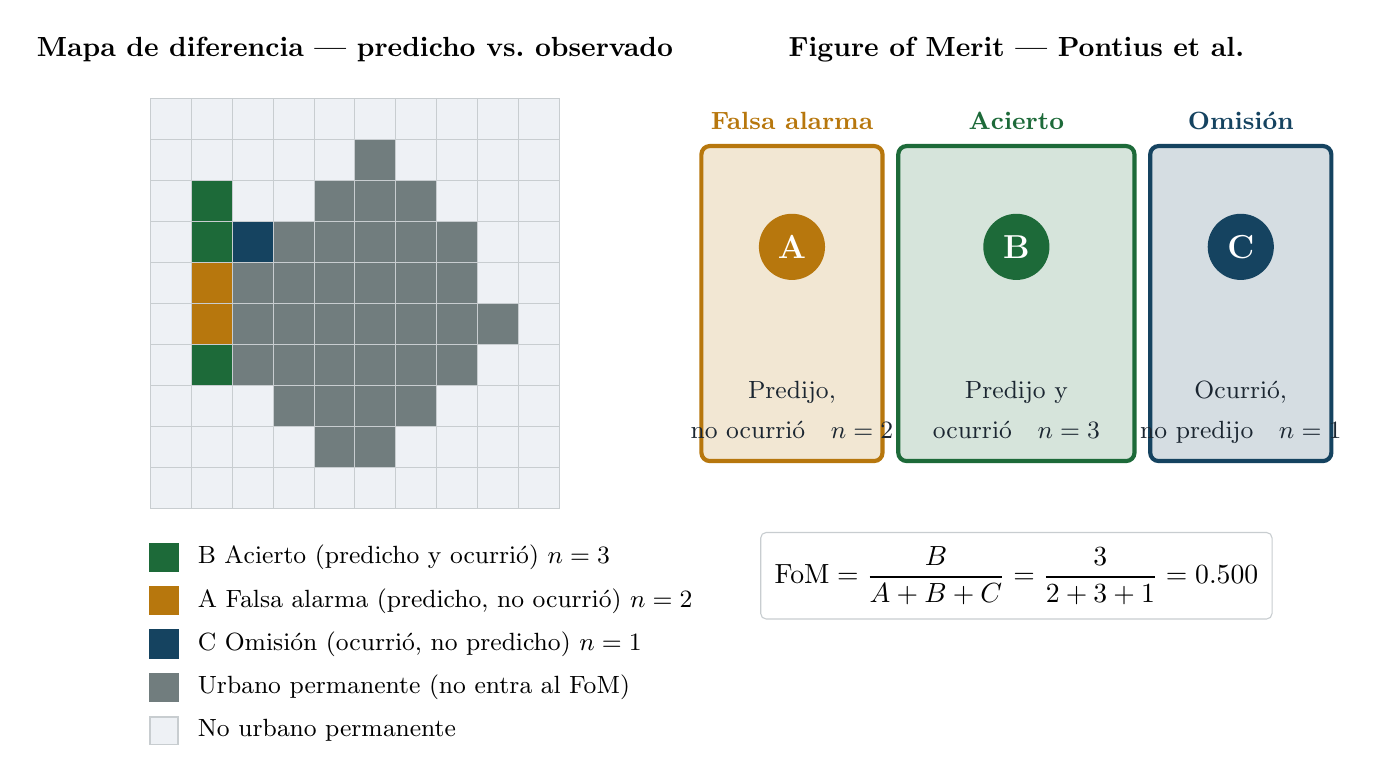
\begin{tikzpicture}[font=\sffamily]
  % — grid background
  \fill[CNU] (0.0000cm,0.0000cm) rectangle (5.2000cm,5.2000cm);
  \fill[CPU] (1.5600cm,2.0800cm) rectangle (2.0800cm,2.6000cm);
  \fill[CPU] (2.0800cm,1.5600cm) rectangle (2.6000cm,2.0800cm);
  \fill[CPU] (2.6000cm,2.0800cm) rectangle (3.1200cm,2.6000cm);
  \fill[CPU] (2.0800cm,3.1200cm) rectangle (2.6000cm,3.6400cm);
  \fill[CPU] (2.6000cm,0.5200cm) rectangle (3.1200cm,1.0400cm);
  \fill[CPU] (2.6000cm,3.6400cm) rectangle (3.1200cm,4.1600cm);
  \fill[CPU] (1.0400cm,2.6000cm) rectangle (1.5600cm,3.1200cm);
  \fill[CPU] (3.6400cm,2.0800cm) rectangle (4.1600cm,2.6000cm);
  \fill[CPU] (3.1200cm,1.0400cm) rectangle (3.6400cm,1.5600cm);
  \fill[CPU] (3.1200cm,2.6000cm) rectangle (3.6400cm,3.1200cm);
  \fill[CPU] (2.0800cm,1.0400cm) rectangle (2.6000cm,1.5600cm);
  \fill[CPU] (2.0800cm,2.6000cm) rectangle (2.6000cm,3.1200cm);
  \fill[CPU] (1.5600cm,1.5600cm) rectangle (2.0800cm,2.0800cm);
  \fill[CPU] (2.6000cm,3.1200cm) rectangle (3.1200cm,3.6400cm);
  \fill[CPU] (1.5600cm,3.1200cm) rectangle (2.0800cm,3.6400cm);
  \fill[CPU] (2.6000cm,1.5600cm) rectangle (3.1200cm,2.0800cm);
  \fill[CPU] (1.0400cm,2.0800cm) rectangle (1.5600cm,2.6000cm);
  \fill[CPU] (3.1200cm,2.0800cm) rectangle (3.6400cm,2.6000cm);
  \fill[CPU] (3.6400cm,1.5600cm) rectangle (4.1600cm,2.0800cm);
  \fill[CPU] (3.1200cm,3.6400cm) rectangle (3.6400cm,4.1600cm);
  \fill[CPU] (3.6400cm,3.1200cm) rectangle (4.1600cm,3.6400cm);
  \fill[CPU] (1.5600cm,1.0400cm) rectangle (2.0800cm,1.5600cm);
  \fill[CPU] (2.0800cm,0.5200cm) rectangle (2.6000cm,1.0400cm);
  \fill[CPU] (2.0800cm,3.6400cm) rectangle (2.6000cm,4.1600cm);
  \fill[CPU] (1.5600cm,2.6000cm) rectangle (2.0800cm,3.1200cm);
  \fill[CPU] (2.6000cm,1.0400cm) rectangle (3.1200cm,1.5600cm);
  \fill[CPU] (2.0800cm,2.0800cm) rectangle (2.6000cm,2.6000cm);
  \fill[CPU] (2.6000cm,2.6000cm) rectangle (3.1200cm,3.1200cm);
  \fill[CPU] (4.1600cm,2.0800cm) rectangle (4.6800cm,2.6000cm);
  \fill[CPU] (2.6000cm,4.1600cm) rectangle (3.1200cm,4.6800cm);
  \fill[CPU] (1.0400cm,1.5600cm) rectangle (1.5600cm,2.0800cm);
  \fill[CPU] (3.1200cm,3.1200cm) rectangle (3.6400cm,3.6400cm);
  \fill[CPU] (3.6400cm,2.6000cm) rectangle (4.1600cm,3.1200cm);
  \fill[CPU] (3.1200cm,1.5600cm) rectangle (3.6400cm,2.0800cm);
  \fill[CHIT] (0.5200cm,3.1200cm) rectangle (1.0400cm,3.6400cm);
  \fill[CHIT] (0.5200cm,3.6400cm) rectangle (1.0400cm,4.1600cm);
  \fill[CHIT] (0.5200cm,1.5600cm) rectangle (1.0400cm,2.0800cm);
  \fill[CFAL] (0.5200cm,2.0800cm) rectangle (1.0400cm,2.6000cm);
  \fill[CFAL] (0.5200cm,2.6000cm) rectangle (1.0400cm,3.1200cm);
  \fill[CMIS] (1.0400cm,3.1200cm) rectangle (1.5600cm,3.6400cm);
  \draw[CBRD,line width=0.35pt,xstep=0.5200cm,ystep=0.5200cm] (0.0000cm,0.0000cm) grid (5.2000cm,5.2000cm);
  \node[font=\normalsize\bfseries,anchor=south] at (2.6000cm,5.5500cm) {Mapa de diferencia --- predicho vs.\ observado};
  \draw[CFAL,fill=CFAL!18,rounded corners=3pt,line width=1.5pt] (7.0000cm,0.6000cm) rectangle (9.3000cm,4.6000cm);
  \node[font=\small\bfseries,text=CFAL,anchor=south] at (8.1500cm,4.6800cm) {Falsa alarma};
  \fill[CFAL] (8.1500cm,3.3200cm) circle (0.42cm);
  \node[font=\large\bfseries,text=white] at (8.1500cm,3.3200cm) {A};
  \node[font=\small,text=CU,anchor=base] at (8.1500cm,1.4000cm) {Predijo,};
  \node[font=\small,text=CU,anchor=base] at (8.1500cm,0.8800cm) {no ocurrió\quad $n=2$};
  \draw[CHIT,fill=CHIT!18,rounded corners=3pt,line width=1.5pt] (9.5000cm,0.6000cm) rectangle (12.5000cm,4.6000cm);
  \node[font=\small\bfseries,text=CHIT,anchor=south] at (11.0000cm,4.6800cm) {Acierto};
  \fill[CHIT] (11.0000cm,3.3200cm) circle (0.42cm);
  \node[font=\large\bfseries,text=white] at (11.0000cm,3.3200cm) {B};
  \node[font=\small,text=CU,anchor=base] at (11.0000cm,1.4000cm) {Predijo y};
  \node[font=\small,text=CU,anchor=base] at (11.0000cm,0.8800cm) {ocurrió\quad $n=3$};
  \draw[CMIS,fill=CMIS!18,rounded corners=3pt,line width=1.5pt] (12.7000cm,0.6000cm) rectangle (15.0000cm,4.6000cm);
  \node[font=\small\bfseries,text=CMIS,anchor=south] at (13.8500cm,4.6800cm) {Omisión};
  \fill[CMIS] (13.8500cm,3.3200cm) circle (0.42cm);
  \node[font=\large\bfseries,text=white] at (13.8500cm,3.3200cm) {C};
  \node[font=\small,text=CU,anchor=base] at (13.8500cm,1.4000cm) {Ocurrió,};
  \node[font=\small,text=CU,anchor=base] at (13.8500cm,0.8800cm) {no predijo\quad $n=1$};
  \node[font=\normalsize\bfseries,anchor=south] at (11.0000cm,5.5500cm) {Figure of Merit --- Pontius et al.};
  \node[draw=CBRD,fill=white,rounded corners=2pt,inner sep=5pt,  font=\normalsize,anchor=north] at (11.0000cm,-0.3000cm) {$\mathrm{FoM}=\dfrac{B}{A+B+C}=\dfrac{3}{2+3+1}=0.500$};
  \fill[CHIT] (0.0000cm,-0.8000cm) rectangle (0.3500cm,-0.4500cm);
  \draw[CHIT,line width=0.6pt] (0.0000cm,-0.8000cm) rectangle (0.3500cm,-0.4500cm);
  \node[font=\small,anchor=west] at (0.4800cm,-0.6250cm) {B Acierto~(predicho y ocurrió)~$n=3$};
  \fill[CFAL] (0.0000cm,-1.3500cm) rectangle (0.3500cm,-1.0000cm);
  \draw[CFAL,line width=0.6pt] (0.0000cm,-1.3500cm) rectangle (0.3500cm,-1.0000cm);
  \node[font=\small,anchor=west] at (0.4800cm,-1.1750cm) {A Falsa alarma~(predicho, no ocurrió)~$n=2$};
  \fill[CMIS] (0.0000cm,-1.9000cm) rectangle (0.3500cm,-1.5500cm);
  \draw[CMIS,line width=0.6pt] (0.0000cm,-1.9000cm) rectangle (0.3500cm,-1.5500cm);
  \node[font=\small,anchor=west] at (0.4800cm,-1.7250cm) {C Omisión~(ocurrió, no predicho)~$n=1$};
  \fill[CPU] (0.0000cm,-2.4500cm) rectangle (0.3500cm,-2.1000cm);
  \draw[CPU,line width=0.6pt] (0.0000cm,-2.4500cm) rectangle (0.3500cm,-2.1000cm);
  \node[font=\small,anchor=west] at (0.4800cm,-2.2750cm) {Urbano permanente (no entra al FoM)};
  \fill[CNU] (0.0000cm,-3.0000cm) rectangle (0.3500cm,-2.6500cm);
  \draw[CBRD,line width=0.6pt] (0.0000cm,-3.0000cm) rectangle (0.3500cm,-2.6500cm);
  \node[font=\small,anchor=west] at (0.4800cm,-2.8250cm) {No urbano permanente};
\end{tikzpicture}
\end{document}
